%%%%%%%%%%%%%%%%%%%%%%%%%%%%%%%%%%%%%%%%%%%%%%%%%%%%%%%%%%%%%%%%%%%%%%%%
% Plantilla TFG/TFM
% Escuela Politécnica Superior de la Universidad de Alicante
% Realizado por: Jose Manuel Requena Plens
% Contacto: info@jmrplens.com / Telegram:@jmrplens
%%%%%%%%%%%%%%%%%%%%%%%%%%%%%%%%%%%%%%%%%%%%%%%%%%%%%%%%%%%%%%%%%%%%%%%%

\chapter{Desarrollo}
\label{desarrollo}
En este capítulo se documenta todo el proceso de desarrollo del proyecto, donde cada sección correspondrá a un sprint. Para cada uno de los sprints, en el primer día se revisará el alcance en Trello y se añadirán nuevas historias a \textit{Backlog}. Asimismo, se llevará a cabo la selección de las historias para implementar dentro del sprint, moviéndolas a la columna \textit{ToDo}.
\section{Sprint 1}
El primer sprint empezó el día 16.03.2026 con la creación del tablero Trello y el repositorio de GitHub. Para el tablero Trello, se han añadido los \textit{Power-Ups} correspondientes a los sprints de Scrum y los puntos de historia de usuario. Los \textit{Power-Ups} son extensiones que permiten añadir nuevas funcionalidades al tablero, como en este caso hacer el seguimiento del sprint y visualizar los puntos de historia de cada una de las tarjetas.
\par Asimismo, se ha procedido a crear las historias de usuario para el Sprint 1, que correspondían a los primeros pasos a implementar dentro de la aplicación. Las historias seleccionadas para el sprint han sido:
\begin{enumerate}
	\item \textbf{001 Walking skeleton:} Como desarrollador, quiero implementar un flujo mínimo que permita comprobar el correcto funcionamiento del programa.  \textbf{5 puntos de historia} \\
	{\small \textit{Criterios de aceptación:}} \\
	Se ha creado una página sencilla en Ionic y Angular. Se comprueba el funcionamiento del login (no registro).
	
	\item \textbf{002 Integración con Supabase:} Como usuario, quiero tener una página de login atractiva y que mis datos y acciones se guarden para la siguiente sesión. Para ello tengo que poder crear mi propia cuenta y poder hacer login. \textbf{3 puntos de historia}
	\\
	{\small \textit{Criterios de aceptación:}}
	\begin{itemize}
		\item El usuario puede registrarse.
		\item El usuario puede iniciar sesión.
		\item El usuario puede editar su perfil.
		\item Sus sesión se guarda en el dispositivo.
	\end{itemize}
	
	\item \textbf{003 Generar sonidos MP3 con Python (básicos):} Como usuario, quiero poder reproducir los sonidos y secuencias musicales correctas para entrenar mi oído. \textbf{5 puntos de historia}
	\\
	{\small \textit{Criterios de aceptación:}} \\
	Se han generado las notas de todas las escalas y se han guardado en assets de la aplicación.
	
	\item \textbf{004 Integración de sonidos MP3 en Ionic con Angular:} Como usuario, quiero que la aplicación reproduzca los sonidos de forma clara para que yo me pueda entrenar. \textbf{1 punto de historia} \\
	{\small \textit{Criterios de aceptación:}} \\
	Los sonidos se guardan en los assets y se reproducen sin errores pulsando un botón.
	
	\item \textbf{005 Estructura del Backend:} Como desarrollador, quiero estructurar mi base de datos para poder organizar todas las entidades, usuarios y lecciones musicales. \textbf{3 puntos de historia} \\
	{\small \textit{Criterios de aceptación:}}
	\begin{itemize}
		\item Diseñar una estructura completa del backend
		\item Crear todas las tablas de BD necesarias.
	\end{itemize}
	
	\item \textbf{006 Servicio de Evaluación de Respuestas:} Como usuario, quiero que mis respuestas sean comparadas con la solución y evaluadas. \textbf{1 punto de historia} \\
	{\small \textit{Criterios de aceptación:}}
	\begin{itemize}
		\item Crear un servicio EvaluacionService para comprobar las respuestas.
		\item Las respuestas se comprueban comunicándose con Supabase.
	\end{itemize}
	
	\item \textbf{007 Modulo de internacionalización i18N:} Como usuario, quiero que la aplicación ofrezca la posibilidad de cambiar el idioma para adaptarse a mi idioma nativo. \textbf{2 puntos de historia} \\
	{\small \textit{Criterios de aceptación:}} \\
	Se han incluido tres módulos de traducciones: Inglés, Castellano, Ucraniano.
\end{enumerate}
\subsection{Historia 005: Estructura del Backend}
La primera tarea que se hizo fue la construcción del entorno de Backend (Historia nº005): empezando con el registro en la plataforma Supabase y acabando con la definición de las tablas, relaciones y reglas de acceso. Las herramientas que proporciona Supabase han sido suficientes para tener el servidor básico en unas 5-6 horas.
\par El diseño UML de la base de datos es el siguiente:
\begin{figure}[H]
	\centering
	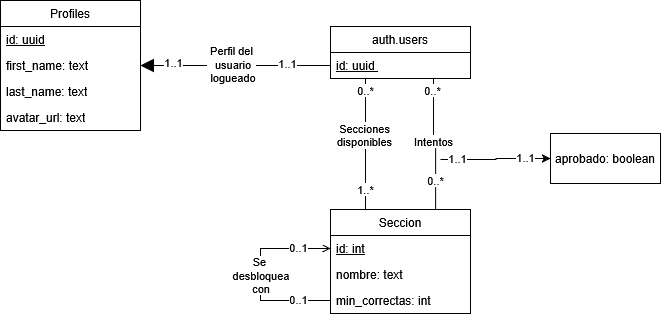
\includegraphics[width=10.5cm]{archivos/bd.drawio.png}
	\caption{Diagrama UML de la estructura de la Base de Datos.}
	\label{fig:bd-uml}
\end{figure}

\subsection{Historia 001: Walking Skeleton}
Esta tarea se refiere a la creación de un proyecto base, el prueba adicional de las herramientas ofrecidas por Angular e Ionic, el uso de los componentes del mismo. Para ello, se ha creado un proyecto ejemplo que es una aplicación de la lista de compra, que muestra el correcto funcionamiento de los servicios y los componentes. El siguiente paso ha sido la implementación de la comunicación entre la aplicación y el servidor. Se ha implementado un módulo básico de inicio de sesión (registro no), para poder comprobar el funcionamiento del login.
\par Por otro lado, se han creado dos páginas para el usuario logeado, una de inicio que muestra una lista de la compra, y la otra que se refiere al perfil del usuario actual.

\subsection{Historia 002: Integración con Supabase}
Esta historia tenía como objetivos mejorar la página de login, implementar la del registro y, por otro lado, finalizar la funcionalidad de la edición de perfil del usuario. Se han creado nuevas tablas SQL auxiliares para almacenar los datos adicionales del usuario que se registra, como es el nombre y apellido. \citep{supabase-user-management-2026}
\begin{figure}[H]
	\centering
	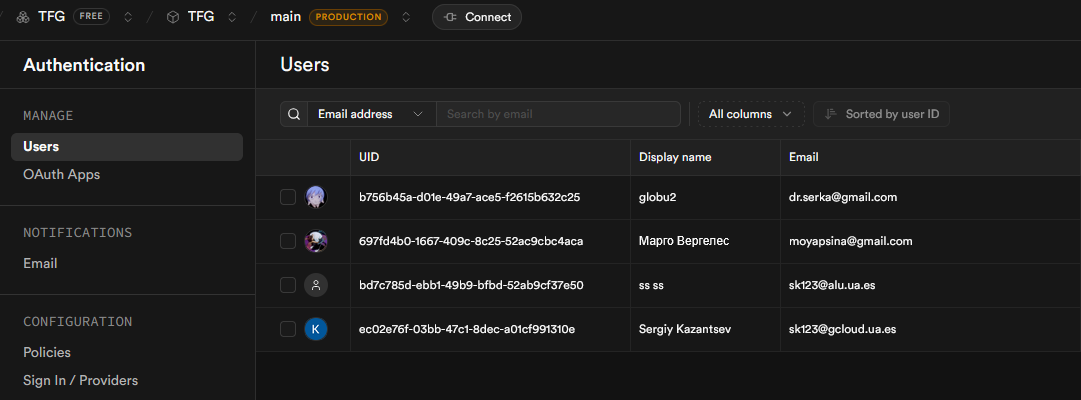
\includegraphics[width=0.7\linewidth]{archivos/screenshot_supabase}
	\caption{Usuarios registrados, vistos dentro de Supabase.}
	\label{fig:screenshotsupabase}
\end{figure}


\subsection{Historia 007: Módulo i18N}
Se ha decidido implementar el módulo de traducciones con antelación para evitar traducir la aplicación cuando esta esté en las fases avanzadas de desarrollo, para así implementar las traducciones gradualmente y disminuir la carga de trabajo. Para las traducciones, se ha usado la biblioteca de Transloco de Angular que permite especificar las traducciones en un fichero JSON.
Las traducciones disponibles en la aplicación serán: el inglés, el castellano y el ucraniano.

\subsection{Historia 006: Servicio de evaluación}
Esta historia tenía como objetivo implementar la comunicación básica entre backend y frontend con el fin de obtener los datos de secciones y ejercicios. Una vez finalizada la historia, pulsando un botón se podía obtener el ejercicio, evaluarlo y registrar el intento.

\subsection{Historia 004: Integración de sonidos}
Para integrar el reproductor de sonidos dentro de la aplicación, se tenía que buscar una librería ligera que permita hacer pre-carga del audio y reproducirlo al pulsar un botón. La librería seleccionada pertenece a la comunidad de Capacitor, el motor de ejecución multiplataforma.

\subsection{Historia 003: Generar sonidos MP3 con Python}
Se ha generado un script de Python que permite generar notas a partir de un fichero Soundfont utilizando el API de MIDI. Para esta aplicación, se han generado todas las notas posibles de las 3 octavas más usadas: la cuarta, quinta y sexta.
\begin{lstlisting}[language=Python, caption=Generación de notas]
	def generate_notes(start_note, end_note):
		for midi_note in range(start_note, end_note + 1):
			midi, piano = create_piano_midi()
			piano.notes.append(
			pm.Note(
				velocity=100,
				pitch=midi_note,
				start=0.0,
				end=1.0
			)
		)
		midi.write(f"{midi_note}.mid")
\end{lstlisting}

\subsection{Burn-up chart del sprint 1.}
\begin{figure}[H]
	\centering
	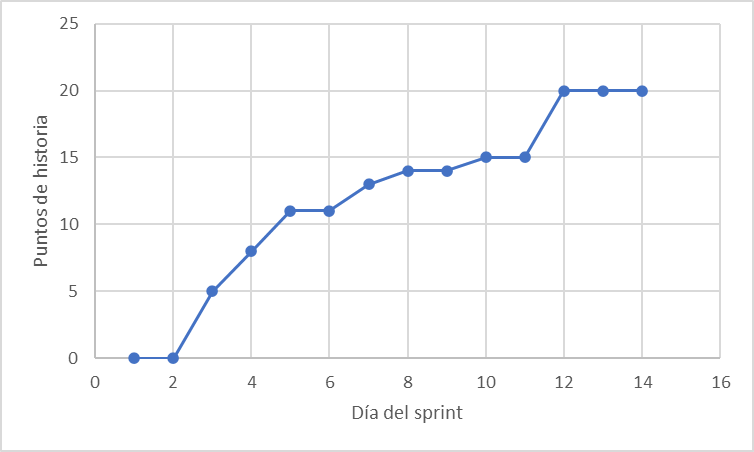
\includegraphics[width=0.8\linewidth]{archivos/sprint1}
	\caption{Burn-up chart del sprint 1.}
	\label{fig:sprint1}
\end{figure}

\section{Sprint 2}
Revisando el progreso del primer sprint, se puede observar un buen progreso de desarrollo e implementación de las historias, aunque ha habido una "meseta" de poco progreso debido al estudio de las otras materias. Por ello, se ha decidido ampliar el volumen de los puntos de historia hasta los 25 puntos, para aprovechar mejor el sprint siguiendo un desarrollo constante.
\par Las historias planificadas para el segundo sprint han sido:
\begin{enumerate}
	\item \textbf{008 Entrenamiento - Reconocimiento de altura:} Como usuario, quiero disponer de una sección de introducción que me permita familiarizar con el sistema y el modo del entrenamiento. \textbf{7 puntos de historia} \\
	{\small \textit{Criterios de aceptación:}} \\
	Se ha creado una sección para el reconocimiento de la altura relativa de las notas. El intento se registra en la parte de Backend y se califica.
	
	\item \textbf{009 Entrenamiento - Reconocimiento del intervalo:} Como usuario, quiero disponer de un módulo que me permita entrenar la habilidad de reconocer los intervalos musicales. \textbf{7 puntos de historia}
	\\
	{\small \textit{Criterios de aceptación:}}
	El usuario puede acceder al módulo. Habrá varias respuestas para cada uno de los ejercicios. El intento se registrará en el Backend y será calificado.
	
	\item \textbf{010 Entrenamiento - Reconocimiento de los tonos y semitonos} Como usuario, quiero disponer de un módulo que me permita entrenar la habilidad de reconocer los tonos y semitonos \textbf{5 puntos de historia}
	\\
	{\small \textit{Criterios de aceptación:}} \\
	El usuario puede acceder al módulo. Habrá varias respuestas para cada uno de los ejercicios. El intento se registrará en el Backend y será calificado.
	
	\item \textbf{011 Generación de sonidos avanzados con Python:} Como usuario, quiero que la aplicación reproduzca los sonidos como los intervalos para que yo pueda entrenarme. \textbf{3 puntos de historia} \\
	{\small \textit{Criterios de aceptación:}} \\
	Los sonidos se guardan en los assets y se reproducen correctamente en los ejercicios.
	
	\item \textbf{012 Diseñar el logotipo y los iconos:} Como usuario, quiero que la aplicación tenga un logotipo/icono para que pueda simpatizar con ella y que pueda distinguirla del resto de las aplicaciones.  \textbf{3 puntos de historia} \\
	{\small \textit{Criterios de aceptación:}} \\
	Se ha diseñado un logotipo que aparecerá como el icono del sitio web y en las aplicaciones de Android.
\end{enumerate}
\subsection{Historia 008: Módulo de reconocimiento de alturas.}
Haciendo uso de las notas generadas en la historia 003, se ha creado el primer módulo introductor que permite al usuario entrenar la capacidad básica del reconocimiento musical. Cada ejercicio se genera de forma aleatoria, seleccionando una nota base y otra a una determinada distancia, de 1 a 10 semitonos.

\par Para poder entender mejor el funcionamiento de los ejercicios que se realizan en la página principal de la aplicación, se proporciona el siguiente diagrama de secuencia:
\begin{figure}[H]
	\centering
	\setlength{\fboxrule}{0.1pt}
	\setlength{\fboxsep}{0pt}
	\fbox{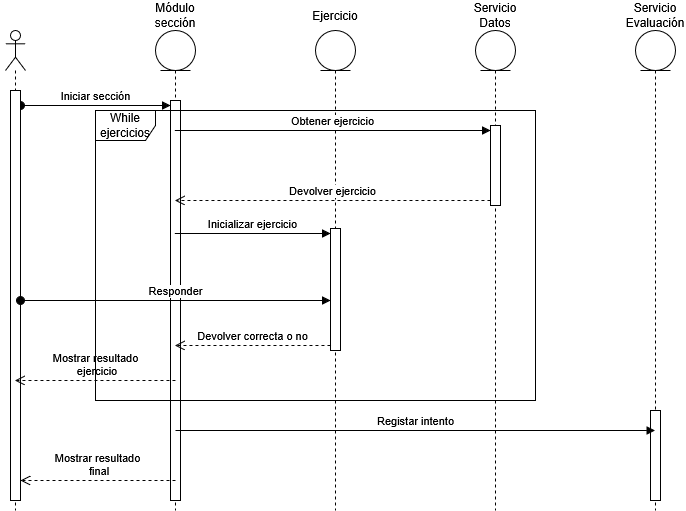
\includegraphics[width=1.0\linewidth]{archivos/diagrama.drawio.png}}
	\caption{Diagrama de secuencia: Realización de una sección.}
	\label{fig:diagrama-secuencia}
\end{figure}
El componente sección es el encargado de inicializar y obtener los datos de cada uno de los ejercicios en el servicio de datos, e itera sobre la colección de ejercicios que obtiene. El servicio de datos genera unas opciones de respuesta aleatorias, obteniendo los audios desde el directorio \textit{Assets}, dependiendo de la sección elegida. 
\par Cada ejercicio, dentro de sí, muestra las opciones de respuesta de forma visual. Una vez que el usuario elige una opción, el evento de respuesta se devuelve al componente padre (Sección), y este componente guarda la cantidad de respuestas correctas.
\par Una vez que se haya llegado a la cantidad necesaria de preguntas respondidas, el intento se registra con la cantidad de respuestas correctas, y, en el caso de que el usuario haya llegado a la nota mínima, se le abre la sección siguiente.

\subsection{Historia 010: Módulo de reconocimiento de los tonos y semitonos.}
Este módulo es la continuación del entrenamiento de reconocimiento de las notas. Esta vez, usando los audios generados previamente, se generan unos ejercicios aleatorios seleccionando una nota base, y la otra de 1 a 2 semitonos de distancia. El objetivo del usuario se determinar esta distancia.

\subsection{Historia 012: Diseñar el logotipo y los iconos.}
Con esta tarea, antes de todo, se ha tenido que pensar en el nombre de la aplicación, su diseño y una mascota que represente la aplicación. Como el nombre, se ha elegido un juego de palabras \textbf{Orcastra}, juntando las palabras Orca y Orquesta. Por lo cual, la paleta de colores de la aplicación será el azul marino, ya que las orcas son animales acuáticos. Por el mismo motivo, el logotipo y el icono de la aplicación será una orca enseñando música en un piano. El logotipo se ha generado usando la herramienta de Canva y posteriormente se ha editado en Photoshop.
\begin{figure}[H]
	\centering
	
\includegraphics[width=0.3\linewidth]{archivos/orca.png}
	\caption{El logotipo de la aplicación}
	\label{fig:orca}
\end{figure}

\subsection{Historia 011: Generación de sonidos avanzados con Python.}
Con esta historia se han generado los intervalos de todas las notas de las octavas cuatro, cinco y seis: más de 450 audios en total. Para ello, se ha usado tanto Python como una aplicación gratuita para editar los archivos \gls{midi}, MuseScore. Como resultado, se han generado los archivos .wav de cada uno de los intervalos. Posteriormente se han comprimido usando FFMPEG al formato .mp3, disminuyendo el tamaño de 250MB hasta >10MB.

\begin{lstlisting}[language=Python, caption=Generación de intervalos]
	def generate_intervals(start_note, intervals, duration=1.0):
		for interval in intervals:
			midi, piano = create_piano_midi()
			piano.notes.append(
				pm.Note(
					velocity=100,
					pitch=start_note,
					start=0.0,
					end=duration
				)
			)
				piano.notes.append(
				pm.Note(
					velocity=100,
					pitch=start_note + interval,
					start=duration,
					end=duration * 2
				)
			)
		
		filename = f"Interval_{start_note}_{interval}.mid"
		midi.write(filename)
\end{lstlisting}

\subsection{Historia 009: Módulo de reconocimiento de intervalos.}
El módulo de reconocimiento de intervalos se ha dividido en tres lecciones separadas, para agilizar el proceso del aprendizaje y enseñar los distintos atributos de los intervalos. La primera lección trata sobre el reconocimiento de los intervalos perfectos: el unísono, cuarta justa, quinta justa y octava. Dentro de la siguiente lección se aprende el reconocimiento de los intervalos mayores y menores, que en total son 8. Finalmente, en la última, el objetivo es reconocer cualquiera de los 12 intervalos posibles.

\subsection{Burn-up chart del sprint 2.}
\begin{figure}[H]
	\centering
	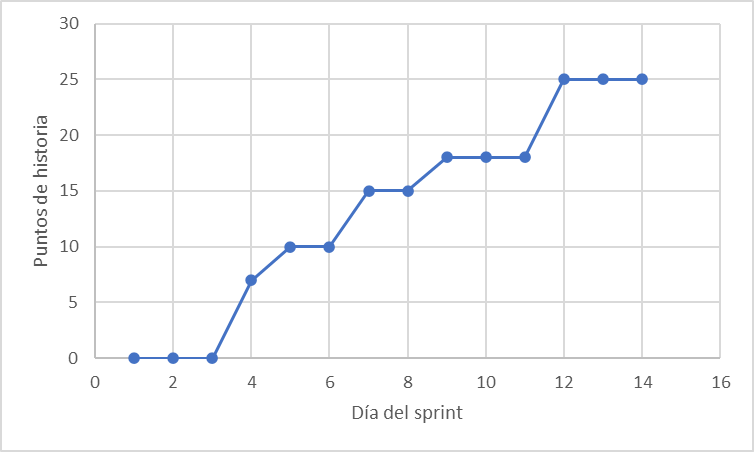
\includegraphics[width=1.0\linewidth]{archivos/screenshot005}
	\caption[Revisión]{Burn-up chart del sprint 2.}
	\label{fig:screenshot005}
\end{figure}

\section{Revisión de los sprints 1 y 2.}
La aplicación tras un mes de desarrollo presenta varias funcionalidades esenciales de la aplicación, quedando por implementar el entrenamiento del reconocimiento de las escalas, acordes y ritmo. Por otro lado, también hace falta mejorar el diseño visual de la aplicación y hacerlo más atractivo. El resultado de los dos sprints es el siguiente:
\begin{figure}[H]
	\centering
	% Control the border thickness and padding
	\setlength{\fboxrule}{0.3pt} % Thickness of the contour
	\setlength{\fboxsep}{0pt}    % Space between image and contour (0pt for tight fit)
	
	\begin{subfigure}{0.4\linewidth}
		\centering
		\fbox{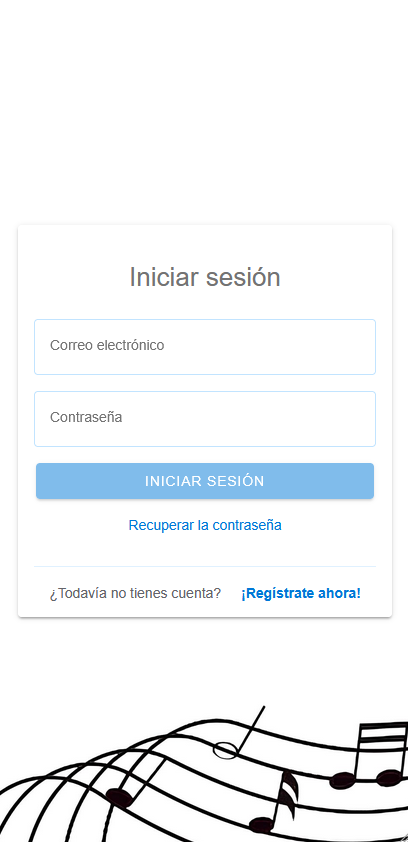
\includegraphics[width=0.5\linewidth]{archivos/screenshot001}}
		\caption[Página de inicio de sesión]{Página de inicio de sesión}
		\label{fig:screenshot001}
	\end{subfigure}
	\hfill 
	\begin{subfigure}{0.4\linewidth}
		\centering
		\fbox{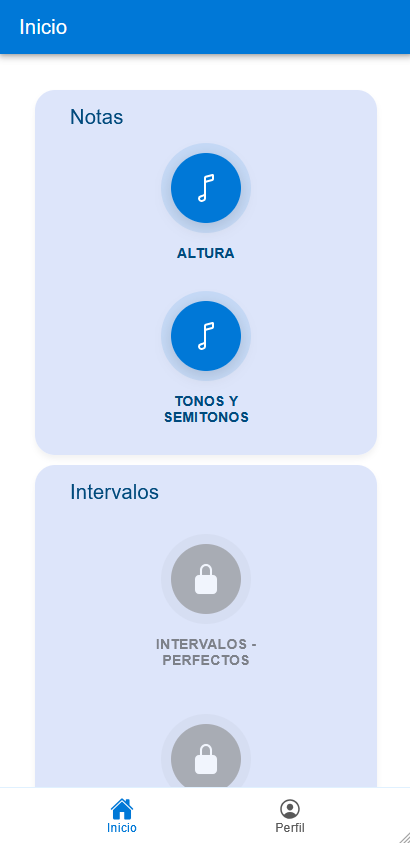
\includegraphics[width=0.5\linewidth]{archivos/screenshot002}}
		\caption[Página de inicio]{Página principal}
		\label{fig:screenshot002}
	\end{subfigure}

	\caption{Pantallas vistas desde el móvil}
\end{figure}

\begin{figure}[H]
	\centering
	\setlength{\fboxrule}{0.3pt} % Made slightly thicker so it's visible
	\setlength{\fboxsep}{0pt}    
	
	\begin{subfigure}{0.4\linewidth}
		\centering
		% Wrap the command here:
		\fbox{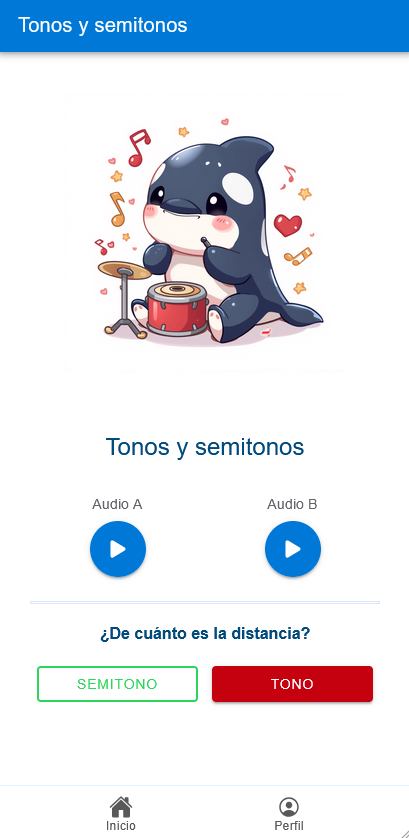
\includegraphics[width=0.5\linewidth]{archivos/screenshot003}}
		\caption[Página de la lección]{Página de la lección de tonos y semitonos}
		\label{fig:screenshot003}
	\end{subfigure}
	\hfill 
	\begin{subfigure}{0.4\linewidth}
		\centering
		% And wrap it here:
		\fbox{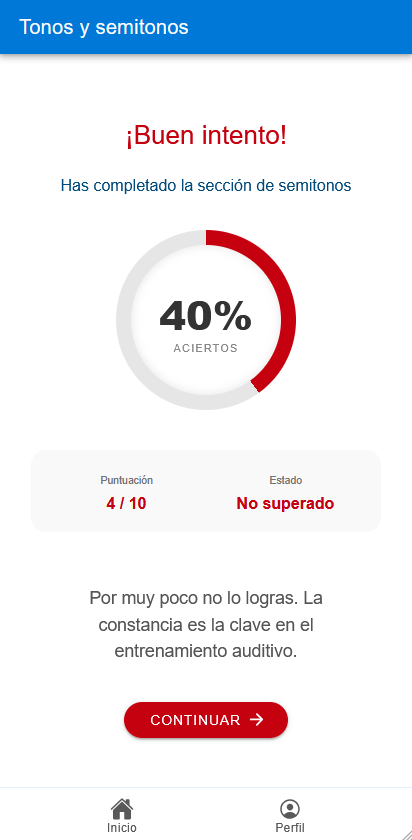
\includegraphics[width=0.5\linewidth]{archivos/screenshot004}}
		\caption[Página de resultados]{Página de los resultados del ejercicio.}
		\label{fig:screenshot004}
	\end{subfigure}
	
	\caption{Pantallas vistas desde el móvil: Ejercicios}
\end{figure}

\newpage
\section{Sprint 3}
Para este sprint se han seleccionado tanto las historias relacionadas con el entrenamiento, como las que mejorarán la experiencia del usuario en otros aspectos de la aplicación. Esto permitirá que nuestro proyecto sea atractivo y fácil de usar por parte del usuario.
\par Las historias planificadas para el tercer sprint han sido:
\begin{enumerate}
	\item \textbf{013 - Login a través de OAuth (Google):} Como usuario, quiero poder registrarme e iniciar sesión usando mi cuenta de Google, para acelerar el proceso.\textbf {3 puntos de historia} \\
	{\small \textit{Criterios de aceptación:}} \\
	Se ha creado la opción "Iniciar sesión con Google" en la página de inicio de sesión.
	
	\item \textbf{014 - Módulo de reconocimiento de escalas:} Como usuario, quiero disponer de un módulo que me permita entrenar la habilidad de reconocer las escalas musicales. \textbf{7 puntos de historia}
	\\
	{\small \textit{Criterios de aceptación:}}
	El usuario puede acceder al módulo. Habrá varias respuestas para cada uno de los ejercicios. El intento se registrará en el Backend y será calificado.
	
	\item \textbf{015 - Módulo de reconocimiento de acordes} Como usuario, quiero disponer de un módulo que me permita entrenar la habilidad de reconocer los acordes. \textbf{5 puntos de historia}
	\\
	{\small \textit{Criterios de aceptación:}} \\
	El usuario puede acceder al módulo. Habrá varias respuestas para cada uno de los ejercicios. El intento se registrará en el Backend y será calificado.
	
	\item \textbf{016 Recuperación de la contraseña olvidada:} Como usuario, quiero que en el caso de que se me olvide la contraseña, pueda establecer una nueva  \textbf{3 puntos de historia} \\
	{\small \textit{Criterios de aceptación:}} \\
	Se ha creado la opción "Recuperar contraseña" en la página de inicio de sesión.
	
	\item \textbf{017 Generación de sonidos (escalas y acordes, con Python):} Como usuario, quiero que la aplicación reproduzca los sonidos como las escalas y acordes para que yo pueda entrenarme. \textbf{5 puntos de historia} \\
	{\small \textit{Criterios de aceptación:}} \\
	Los sonidos se guardan en los assets y se reproducen correctamente en los ejercicios.
	
	\item \textbf{018 Mejorar la UI:} Como usuario, quiero que la aplicación sea agradable de usar tanto en el móvil como en el navegador  \textbf{2 puntos de historia.}
	{\small \textit{Criterios de aceptación:}} \\
	Se han actualizado las páginas de Inicio y Perfil de usuario.
	
\end{enumerate}
\subsection{Historia 013: Login a través de OAuth (Google).}
Para realizar la tarea, se han creado dos clientes (Web y Android) usando Google Cloud, que permite la integración de OAuth con Supabase. El ID de los clientes se usa en el frontend, se pasa a Supabase y se compara con el ID de Google Cloud. De momento se ha implementado para pruebas en local, dado que la aplicación no se ha desplegado. \citep{capgo, supabase-google-login-2026}
\begin{figure}
	\centering
	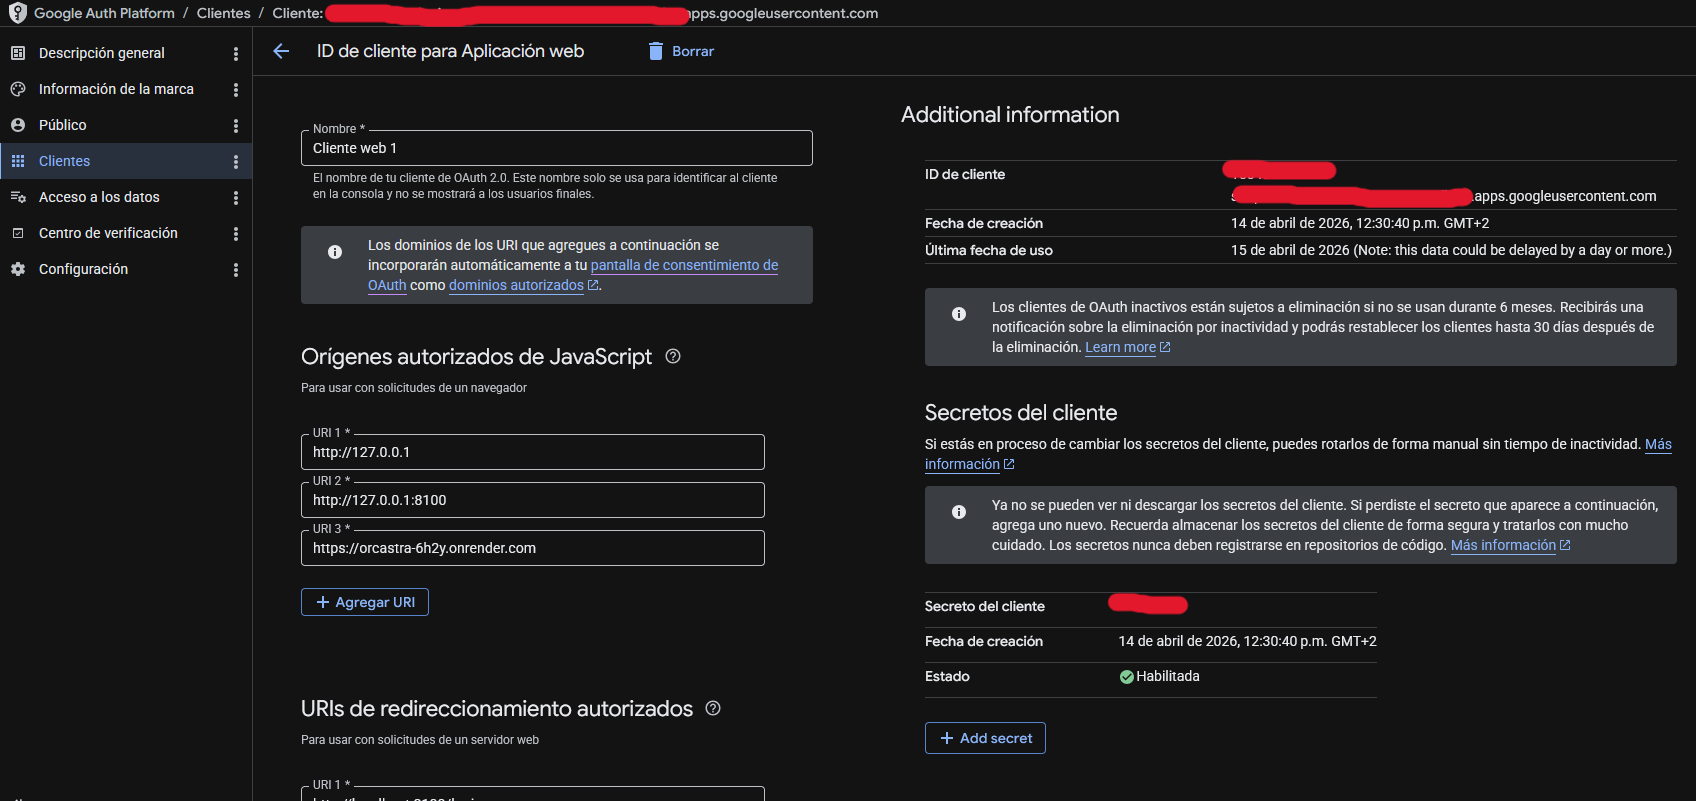
\includegraphics[width=1.0\linewidth]{archivos/screenshot010}
	\caption{Consola de Google Cloud, implementación del cliente Web.}
	\label{fig:screenshot010}
\end{figure}

\subsection{Historia 017: Generación de sonidos (escalas y acordes, con Python).}
Se han generado los sonidos de las escalas y acordes más importantes. Por otro lado, también se han añadido las escalas que se reproducen con la mitad de la velocidad de las originales, y, también, los audios que reproduce cada nota de un acorde secuencialmente. Esto permite hacer el ejercicio más fácil y fomentar el aprendizaje. Adicionalmente, todos los audios se han comprimido usando FFMPEG.

\subsection{Historia 016: Recuperación de la contraseña olvidada.}
El cambio de contraseña se ha implementado usando el servidor SMTP propio de Supabase que permite enviar hasta 2 correos electrónicos cada hora. Cada correo incluye un token de un solo uso que permite resetear la contraseña y posteriormente iniciar sesión.

\subsection{Historia 014: Módulo de reconocimiento de escalas}
El módulo implementado se ha dividido en tres lecciones: la primera sirve para aprender a distinguir entre las escalas mayores y menores, la segunda para distinguir distintos tipos de escalas menores, y en la tercera el objetivo es reconocer todas las escalas, tanto la escala mayor como las menores. Por otro lado, el módulo facilita el aprendizaje introduciendo una nueva funcionalidad de reproducción de audio. La primera vez que se reproduce, esto se hace a una velocidad normal; si el usuario quiere escuchar el audio de nuevo, se reproduce a una velocidad menor (el doble de tiempo). 

\subsection{Historia 015: Módulo de reconocimiento de acordes}
El objetivo de este módulo es aprender a distinguir los distintos acordes, que pueden ser: Mayor, Menor, Aumentado, Disminuido. Como son pocos, se ha implementado todo el programa en una sola lección. Al igual que el módulo anterior, incorpora una funcionalidad que pretende mejorar la experiencia de usuario a la hora de realizar el ejercicio. La primera vez que se escucha el acorde, suena como debería: todas las notas al mismo tiempo. Sin embargo, la segunda vez, el acórde se "rompe" y las notas se reproducen secuencialmente.

\subsection{Historia 018: Mejorar la UI}
Debido a que la aplicación se implementa tanto para Web como para Android, tiene que ser agradable para las dos plataformas. Dado que Ionic es un framework orientado principalmente a móviles, se tenían que realizar algunos ajustes para mejorar la interfaz en la Web. Sin embargo, también se han cambiado otros aspectos de la aplicación, como la introducción de nuevos colores para permitir distinguir las opciones; por otro lado, se ha cambiado la página del perfil del usuario. El resultado final ha sido el siguiente:
\begin{figure}[H]
	\setlength{\fboxrule}{0.3pt} % Made slightly thicker so it's visible
	\setlength{\fboxsep}{0pt} 
	\centering
	\fbox{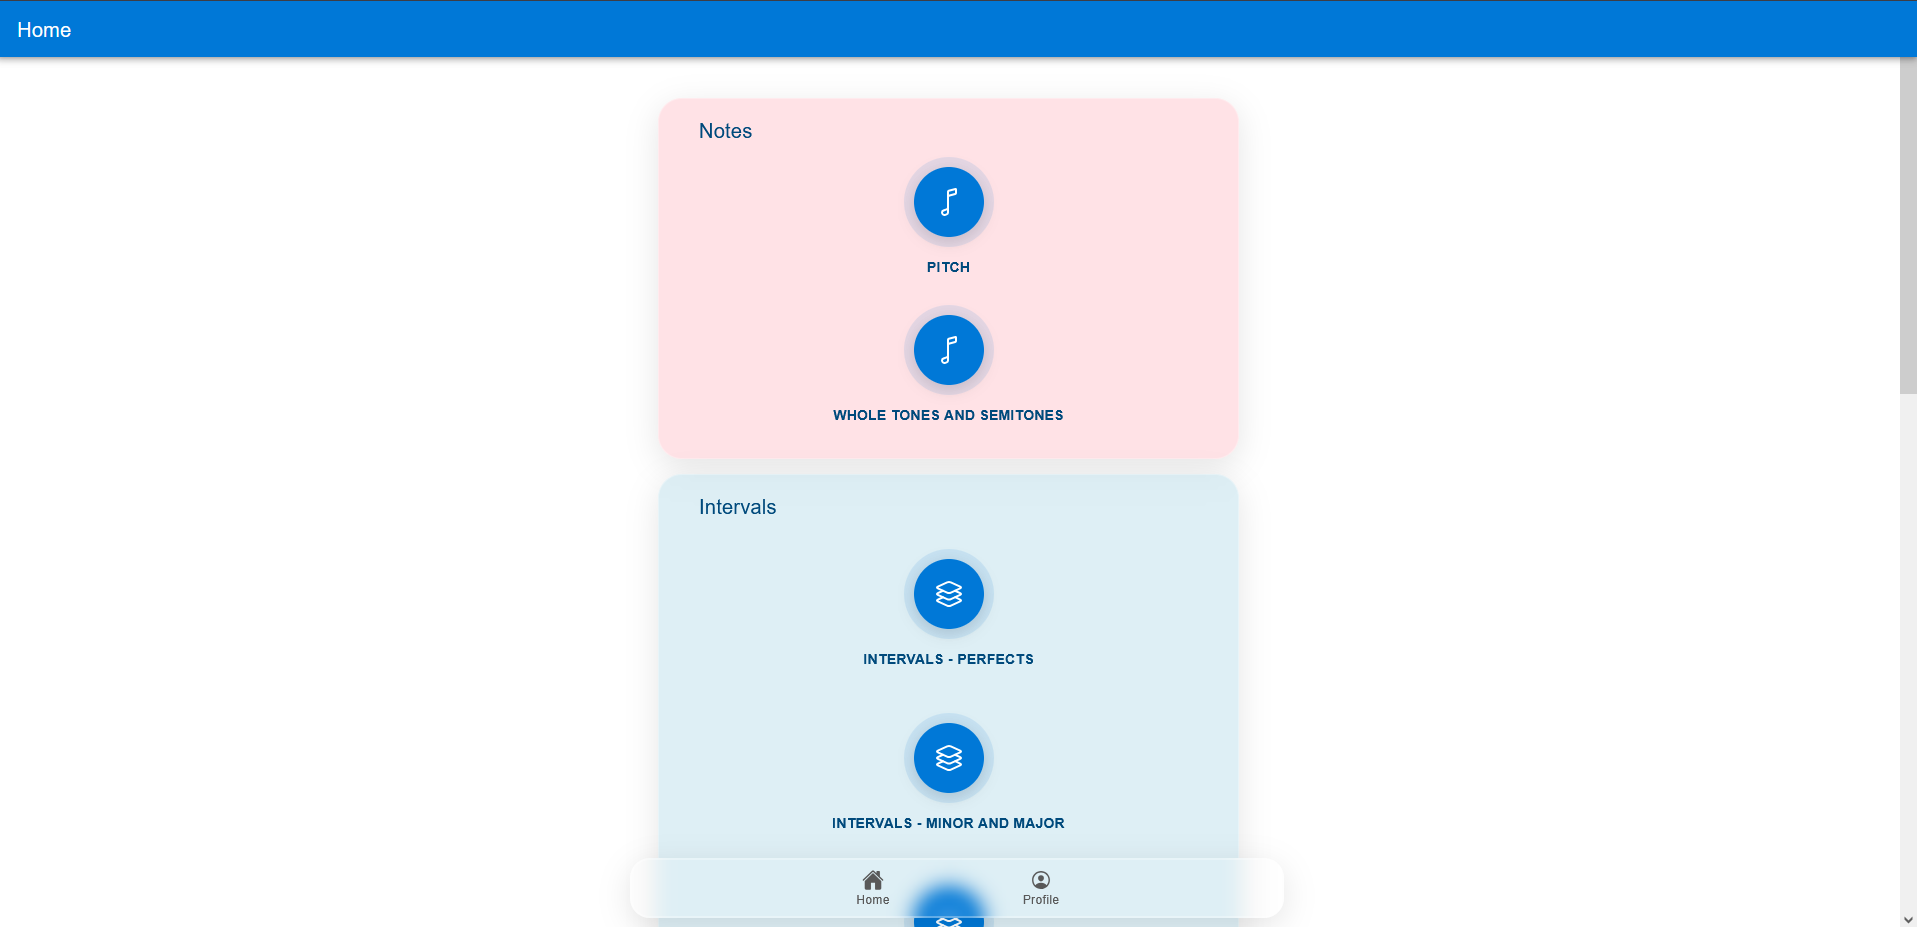
\includegraphics[width=0.8\linewidth]{archivos/screenshot006}}
	\label{fig:screenshot006}
	\caption{Pantalla principal actualizada (Web)}
\end{figure}

\begin{figure}[H]
	\centering
	\setlength{\fboxrule}{0.3pt} % Made slightly thicker so it's visible
	\setlength{\fboxsep}{0pt}
	\begin{subfigure}{0.4\linewidth}
		\centering
		% Wrap the command here:
		\fbox{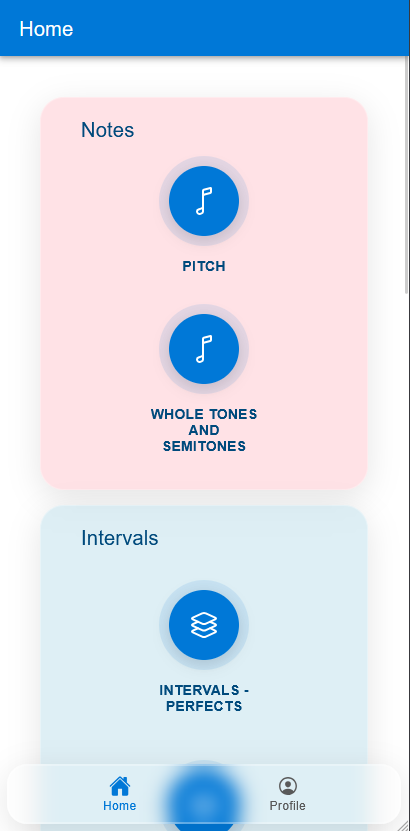
\includegraphics[width=0.45\linewidth]{archivos/screenshot007}}
		\label{fig:screenshot007}
		\caption{Pantalla principal}
	\end{subfigure}
	\hfill 
	\begin{subfigure}{0.4\linewidth}
		\centering
		% And wrap it here:
		\fbox{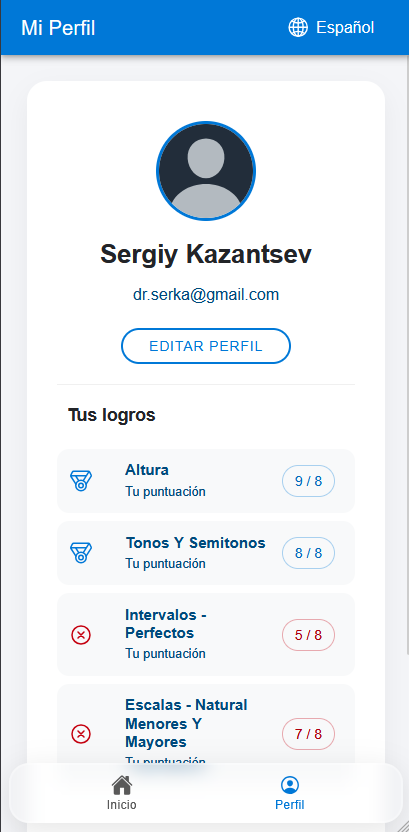
\includegraphics[width=0.45\linewidth]{archivos/screenshot008}}
		\label{fig:screenshot008}
		\caption{Pantalla del perfil del usuario}
	\end{subfigure}
	\caption{Pantallas actualizadas (Android)}
\end{figure}

\subsection{Burn-up chart del sprint 3.}
\begin{figure}[H]
	\centering
	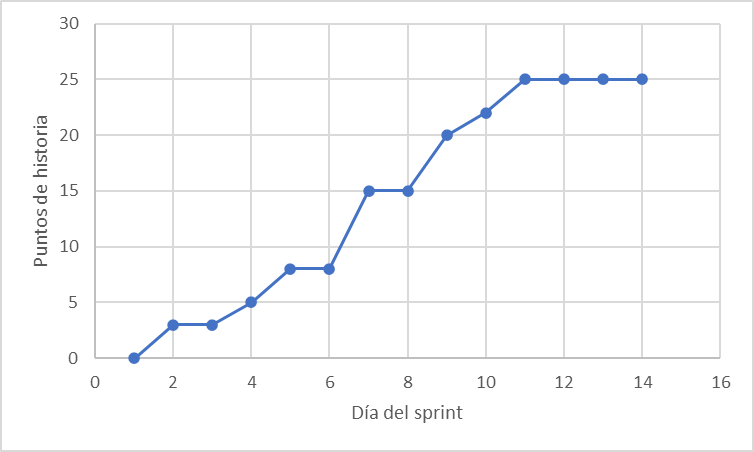
\includegraphics[width=1.0\linewidth]{archivos/screenshot009}
	\caption{Burn-up chart del sprint 3.}
	\label{fig:screenshot009}
\end{figure}
\newpage
\section{Sprint 4}
Este sprint, dado que es uno de los finales, incorporará distintas mejoras de la \gls{ux} y arreglos de bugs y errores. También se desarrollarán nuevas funcionalidades relacionadas con el aprendizaje. Por otro lado, la cantidad de los puntos de historia planificados se expande hasta 30 puntos para abordar todas las funcionalidades planificadas.
\par Las historias planificadas para el cuarto sprint han sido:
\begin{enumerate}
	\item \textbf{019 - Botón de compartir resultados:} Como usuario, quiero poder compartir mis resultados con mis compañeros o con mi profesor de música.\textbf {1 punto de historia} \\
	{\small \textit{Criterios de aceptación:}} \\
	Se ha creado un botón "Compartir resultados" al finalizar una lección. Se podrá compartir a través de redes sociales una imagen que incluirá la fecha y el nombre del usuario.
	
	\item \textbf{020 - Entrenador libre:} Como usuario, quiero tener la opción de entrenarme para poder prepararme ante una lección. \textbf{7 puntos de historia}
	\\
	{\small \textit{Criterios de aceptación:}}
	Se ha creado una página "Entrenador libre" que le permite al usuario seleccionar la categoría que quiere entrenar, y los distintos ajustes dependiendo de la categoría. Por ejemplo, en la categoría "Escalas" podrá seleccionar qué escalas quiere que entren a los ejercicios y cuáles no.
	
	\item \textbf{021 - Generación de sonidos: Ritmos (Python)} Como usuario, quiero que la aplicación tenga suficientes sonidos para poder reconocer los ritmos. \textbf{5 puntos de historia}
	\\
	{\small \textit{Criterios de aceptación:}} \\
	El usuario puede acceder al módulo. Habrá varias respuestas para cada uno de los ejercicios. El intento se registrará en el Backend y será calificado.
	
	\item \textbf{022 - Módulo de reconocimiento de ritmos:} Como usuario, quiero tener un módulo que me permita entrenar los ritmos.  \textbf{7 puntos de historia} \\
	{\small \textit{Criterios de aceptación:}} \\
	Se ha creado el módulo de reconocimiento de ritmos.
	
	\item \textbf{023 - Página de entrenamiento del oído perfecto:} Como usuario, quiero tener una herramienta que me permita entrenar mi oído perfecto.  \textbf{7 puntos de historia} \\
	{\small \textit{Criterios de aceptación:}} \\
	Se ha creado una nueva página que incorpora el reconocimiento de una nota en el teclado del piano.
	
	\item \textbf{024 - Pruebas y arreglos:} Como usuario, quiero que la aplicación sea lo más intuitiva posible y que no haya errores ni bugs que afecten a mi experiencia. \textbf{7 puntos de historia} \\
	{\small \textit{Criterios de aceptación:}} \\
	Realizar pruebas manuales exhaustivas, implicando voluntarios probadores.
\end{enumerate}

\subsection{Historia 019: Botón de compartir resultados}
Se ha añadido la opción de compartir los resultados una vez terminado el intento de una sección. En la página de los resultados, también se ha añadido el nombre del usuario y la fecha de la realización para identificar el intento: servirá para compartirlo con los amigos, con el profesor de la escuela de música. La biblioteca usada convierte la página HTML en una imagen PNG, y el módulo de capacitor se encarga del API que permite compartir la imagen a través de las redes sociales. Por otro lado, la funcionalidad de compartir los resultados en el navegador descarga la imagen en el ordenador y permite que el usuario la maneje.

\subsection{Historia 020: Entrenador libre}
La nueva funcionalidad importante de la aplicación es el entrenador libre. Permitirá que el usuario pueda repasar los conocimientos y/o entrenarse antes de enfrentarse a las pruebas de la página principal. Esto permitirá que el usuario tenga menos presión a la hora de realizar los ejercicios, sabiendo que si está en el modo libre su intento no se evaluará.

\subsection{Historia 023: Entrenamiento del oído perfecto}
Se ha creado una nueva página, que junto al entrenador libre, permitirá al usuario entrenar los conceptos más difíciles de una forma que le haga menos estrés que la realización de las pruebas evaluadas. Dado que la página pretende entrenar el oído perfecto, se ha simplificado al máximo. El usuario dispone de 2 reproducciones del audio, despues de las cuales, ha de identificar la nota en un teclado del piano. El teclado es interactivo y permite escuchar la nota antes de elegirla. 

\subsection{Historia 021: Generación de sonidos -  Ritmos (Python)}
Se ha generado los ritmos 4/4 que incluyen notas y silencios de distintas longitudes. Cada audio incluye un metrónomo para dar el ritmo, seguido por las notas que el usuario tendrá que identificar. 

\subsection{Historia 022: Módulo de reconocimiento de ritmos}
Se ha creado el nuevo módulo de reconocimiento, innovativo respecto al rest de la aplicación. Para identificar cada secuencia de notas se utiliza una forma de aprendizaje que se denomina "dictado musical rítmico". Dentro de este ejercicio, el objetivo del alumno es escuchar la secuencia e intentar repetirla dado un conjunto de notas. La forma final de la sección es la siguiente:
\begin{figure}[H]
	\centering
	\setlength{\fboxrule}{0.3pt} % Made slightly thicker so it's visible
	\setlength{\fboxsep}{0pt}
	\begin{subfigure}{0.35\linewidth}
		\centering
		% Wrap the command here:
		\fbox{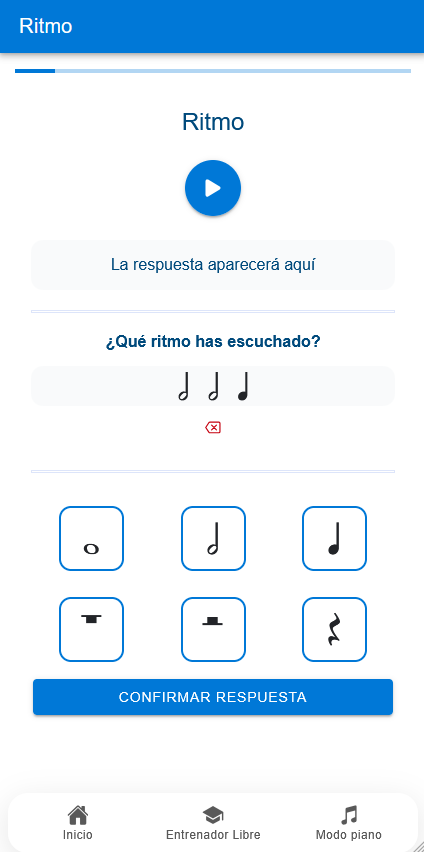
\includegraphics[width=0.7\linewidth]{archivos/screenshot011}}
		\label{fig:screenshot011}
		\caption{}
	\end{subfigure}
	\hfill 
	\begin{subfigure}{0.35\linewidth}
		\centering
		% And wrap it here:
		\fbox{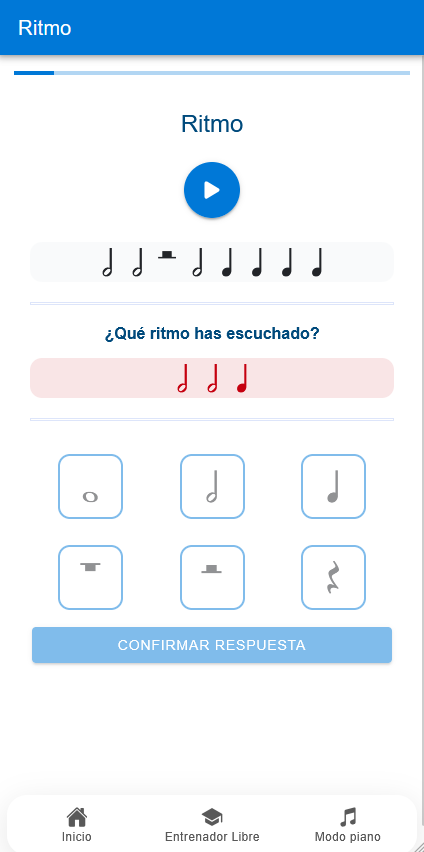
\includegraphics[width=0.7\linewidth]{archivos/screenshot012}}
		\label{fig:screenshot012}
		\caption{}
	\end{subfigure}
	\caption{Pantallas del ejercicio de ritmos (Android)}
\end{figure}

\subsection{Historia 023: Mejoras y arreglos de bugs}
Dentro de esta historia se han buscado distintos errores/bugs e inconsistencias de la interfaz del usuario. Para ello, se ha optado por la realización de las pruebas manuales involucrando personas voluntarias que han comentado su experiencia sobre su experiencia de uso de la aplicación. Se han arreglado los errores de reproducción de los audios, también distintas inconsistencias e incompatibilidades entre las dos plataformas.

\subsection{Burn-up chart del sprint 4.}
\begin{figure}[H]
	\centering
	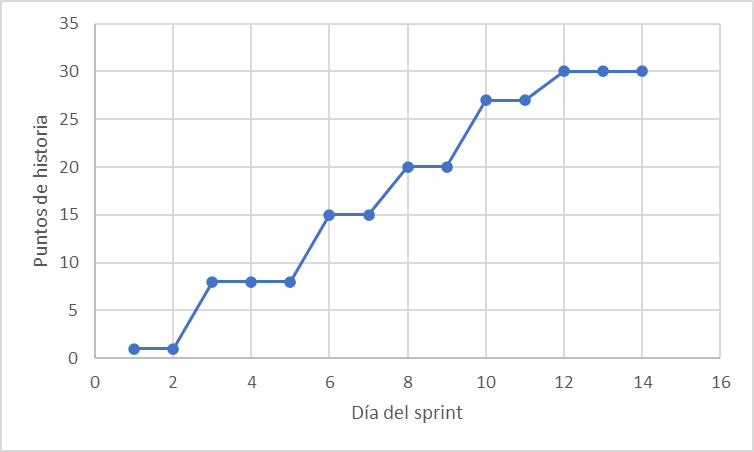
\includegraphics[width=0.6\linewidth]{archivos/screenshot013}
	\caption{Burn-up chart del sprint 4.}
	\label{fig:screenshot013}
\end{figure}

\section{Mejoras finales}
Antes de mostrar los resultados, cabe mencionar las distintas mejoras que no se han comentado durante el proceso de desarrollo; algunas de ellas se han implementado para facilitar la realización de alguna historia de usuario, otras se han hecho con el fin de mejorar la seguridad o la experiencia del usuario. Todas las mejoras se han considerado importantes para mencionarlas una vez alcanzados los objetivos generales.
\subsection{Captcha}
Se ha implementado la protección contra bots/verificación del usuario a través del uso de hCaptcha, integrando esta herramienta con API interna de Supabase. Para ello, se ha creado un proyecto en el sitio de hCaptcha, obteniendo, por un lado, un código público, y por otro, un secreto que se guarda en Supabase. Como resultado, todas las llamadas de inicio de sesión, registro y restablecimiento de contraseña requieren un token que se obtiene al completar un Captcha. \citep{supabase-captcha-2026, hcaptcha-2026}
\begin{figure}[H]
	\centering
	\setlength{\fboxrule}{0.3pt} % Made slightly thicker so it's visible
	\setlength{\fboxsep}{0pt}
	\begin{subfigure}{0.30\linewidth}
		\centering
		% Wrap the command here:
		\fbox{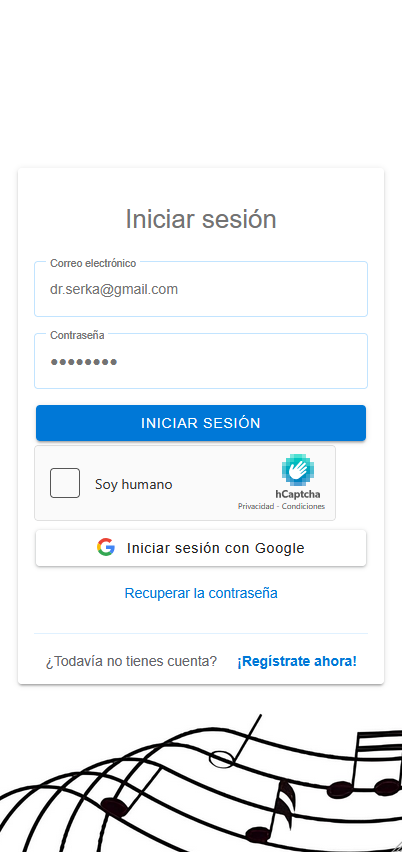
\includegraphics[width=0.7\linewidth]{archivos/screenshot014}}
		\label{fig:screenshot014}
		\caption{}
	\end{subfigure}
	\hfill 
	\begin{subfigure}{0.30\linewidth}
		\centering
		% And wrap it here:
		\fbox{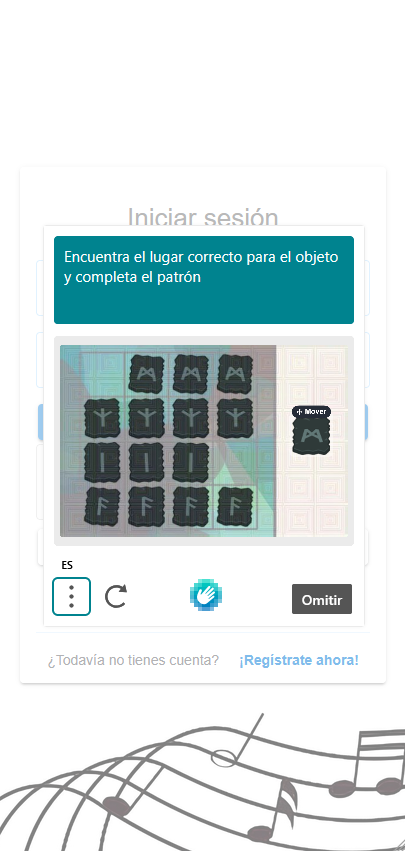
\includegraphics[width=0.7\linewidth]{archivos/screenshot015}}
		\label{fig:screenshot015}
		\caption{}
	\end{subfigure}
	\caption{Verificación Captcha al iniciar sesión (Android)}
\end{figure}
\subsection{Logros del usuario}
Para que el usuario pueda hacer un mejor seguimiento del progreso, a mediados del sprint 4, en la página del perfil se ha implementado una sección de logros del usuario, que muestra el mejor resultado dentro de cada lección y comparado con la nota mínima que se tiene que obtener. Si el resultado del usuario es mayor o igual a la nota mínima, se le muestra una medalla. Si no se ha conseguido alcanzar la nota mínima, el mejor intento se muestra en rojo. El resultado ha sido el siguiente:
\begin{figure}[H]
	\centering
	\setlength{\fboxrule}{0.3pt}
	\setlength{\fboxsep}{0pt}
	\fbox{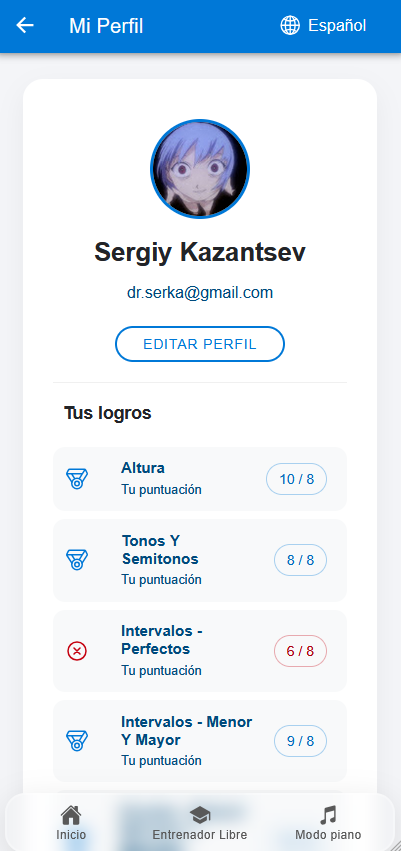
\includegraphics[width=0.2\linewidth]{archivos/screenshot016}}
	\caption{Logros del usuario\protect\footnotemark}
	\label{fig:screenshot016}
\end{figure}
\footnotetext{Debido a que es un usuario de prueba, las secciones no han sido abiertas en el orden progresivo como habría sido en el caso de un usuario real.}
\subsection{Guías para el entrenador libre y el modo piano}
Debido a que el entrenador libre y el modo piano no resultaban tan intuitivos en comparación con los ejercicios principales, se ha decidido crear una pequeña guía a la cual un usuario puede acceder en cualquier momento. Para ello, se ha añadido un botón con icono del signo de interrogación, al pulsar el cual se muestra una ventana explicando el funcionamiento del módulo. Dentro de la aplicación, se ve de la siguiente manera:
\begin{figure}[H]
	\centering
	\setlength{\fboxrule}{0.3pt} % Made slightly thicker so it's visible
	\setlength{\fboxsep}{0pt}
	\begin{subfigure}{0.38\linewidth}
		\centering
		% Wrap the command here:
		\fbox{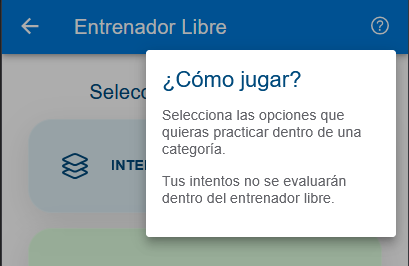
\includegraphics[width=0.7\linewidth]{archivos/screenshot017}}
		\label{fig:screenshot017}
		
	\end{subfigure}
	\hfill 
	\begin{subfigure}{0.38\linewidth}
		\centering
		% And wrap it here:
		\fbox{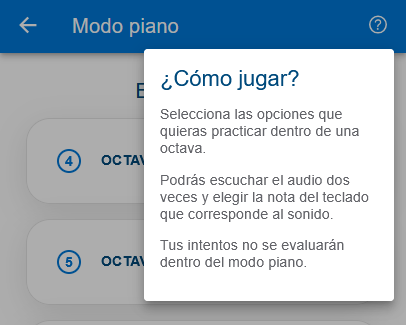
\includegraphics[width=0.7\linewidth]{archivos/screenshot018}}
		\label{fig:screenshot018}
	\end{subfigure}
	\caption{Guías para los modos no evaluables.}
\end{figure}

%\section{Inserción de código}

%A veces tendrás que insertar algún pedazo de código fuente para explicar algo relacionado con él. No sustituyas explicaciones con códigos enormes. Si pones algo de código en tu TFG que sea para demostrar algo o explicar alguna solución.
%
%\LaTeX~te ayuda a escribir código de manera que su presentación tenga las marcas y tabulaciones propias de este tipo de texto. Para ello, debes poner el código que escribas DENTRO de un entorno  que se llama ``listings''.  La plantilla ya tiene una serie de instrucciones para incluir el paquete ``listings'' y añadirle algunos modificadores por lo que no tienes que incluirlo tú. Simplemente, mete tu código en el entorno ``lstlisting'' y ya está. Puedes indicar el lenguaje en el que está escrito el código y así \LaTeX~lo mostrará mejor. 
%\\
%\par En el archivo \textit{estiloscodigoprogramacion.tex} están definidos algunos lenguajes para mostrarlos con un diseño concreto, se pueden modificar para cambiar el coloreado del código, qué términos se ponen en negrita, etc.
%Si se quiere profundizar más en la función ``listings'' se puede consultar su manual en \url{http://osl.ugr.es/CTAN/macros/latex/contrib/listings/listings.pdf}, aunque hay mucha información en foros y blog's que es más fácil de comprender.
%
%\par Veamos un ejemplo en la figura \ref{C_code}:
%
%\begin{lstlisting}[style=Latex-color]
%\begin{lstlisting}[style=C, caption={ejemplo código C},label=C_code]
%	#include <stdio.h>
%	int main(int argc, char* argv[]) {
%  	puts("Hola mundo!");
%	}
%\ end{lstlisting}	
%\end{lstlisting}
%
%El resultado será:
%\begin{lstlisting}[style=C, caption={ejemplo código C},label=C_code]
%#include <stdio.h>
%// Comentario
%int main(int argc, char* argv[]) {
%  puts("Hola mundo!");
%}
%\end{lstlisting}
%\vspace{1em}
%\noindent\hrule
%\vspace{1em}
%Si lo quieres en color, está definido el estilo C-color en el archivo \textit{estiloscodigoprogramacion.tex}, con algunos parámetros para mejorar la visualización:
%\begin{lstlisting}[style=Latex-color]
%\begin{lstlisting}[style=C-color, caption={ejemplo código C en color},label=C_code-color]
%#include <stdio.h>
%// Comentario
%int main(int argc, char* argv[]) {
%  puts("Hola mundo!");
%}
%\ end{lstlisting}
%\end{lstlisting}
%\begin{lstlisting}[style=C-color, caption={ejemplo código C en color},label=C_code-color]
%	#include <stdio.h>
%	// Comentario
%	int main(int argc, char* argv[]) {
%  	puts("Hola mundo!");
%	}
%\end{lstlisting}
%\vspace{1em}
%\noindent\hrule
%\vspace{1em}
%Por supuesto, puedes mejorar esta presentación utilizando más modificadores. En la sección \ref{usos} se indican algunos detalles.
%
%Otro ejemplo, ahora para mostrar código PHP, sería escribir en tu fichero \LaTeX~lo siguiente:
%\begin{lstlisting}[style=Latex-color,numbers=none]
% \begin{lstlisting}[style=PHP, caption={ejemplo código PHP},label=PHP_code]
% /* 
%Ejemplo de código en PHP para escribir tu primer programa en este lenguaje
%Copia este código en tu ordenador y ejecútalo
%*/
%<html>
%  <head>
%    <title>Prueba de PHP</title>
%  </head>
%  <body>
%    <?php echo '<p>Hola Mundo</p>'; ?> //esto lo escribe TODO el mundo
%  </body>
%</html>
% \ end{lstlisting}
%\end{lstlisting}
% 
% y el resultado es el siguiente:
% 
% \begin{lstlisting}[style=PHP, caption={ejemplo código PHP},label=PHP_code,firstnumber=100]
%/* 
%Ejemplo de código en PHP para escribir tu primer programa en este lenguaje. Copia este código en tu ordenador y ejecútalo
%*/
% <html>
%  <head>
%    <title>Prueba de PHP</title>
%  </head>
%  <body>
%    <?php echo '<p>Hola Mundo</p>'; ?> //esto lo escribe TODO el mundo
%  </body>
%</html>
% \end{lstlisting}
% \vspace{1em}
%\noindent\hrule
%\vspace{1em}
% O también en color: 
% \begin{lstlisting}[style=PHP-color, caption={ejemplo código PHP},label=PHP_code2]
%/* 
%Ejemplo de código en PHP para escribir tu primer programa en este lenguaje. Copia este código en tu ordenador y ejecútalo
%*/
% <html>
%  <head>
%    <title>Prueba de PHP</title>
%  </head>
%  <body>
%    <?php echo '<p>Hola Mundo</p>'; ?> //esto lo escribe TODO el mundo
%  </body>
%</html>
% \end{lstlisting}
% 
% Observa cómo \LaTeX~ha puesto los comentarios en gris y ajustado el código para que se muestre más claro.
%\vspace{1em}
%\noindent\hrule
%\vspace{1em}
% A continuación se muestran otros ejemplos:
% \begin{lstlisting}[style=Matlab-color, caption={ejemplo código Matlab en color},label=Matlab_code]
%%% Code sections are highlighted.
%% System command are supported...
%!touch testFile.txt
%A = [1, 2, 3;... %... as is line continuation.
%     4, 5, 6];
%fid = fopen('testFile.text', 'w');
%for k=1:10
%  fprintf(fid, '%6.2f \n', k)
%end
%x=1; %% this is just a comment, not the start of a section
%% Context-sensitive keywords get highlighted correctly...
%p = properties(person); %(here, properties is a function)
%x = linspace(0,1,101);
%y = x(end:-1:1);
%% ... even in nonsensical code.
%]end()()(((end while {    end    )end ))))end (end
%%{
%    block comments are supported
%%} even
%runaway block comments are
%\end{lstlisting}
%
%\begin{lstlisting}[style=Matlab, caption={ejemplo código Matlab en blanco y negro},label=Matlab_codebn]
%%% Code sections are highlighted.
%% System command are supported...
%!touch testFile.txt
%A = [1, 2, 3;... %... as is line continuation.
%     4, 5, 6];
%fid = fopen('testFile.text', 'w');
%for k=1:10
%  fprintf(fid, '%6.2f \n', k)
%end
%x=1; %% this is just a comment, not the start of a section
%% Context-sensitive keywords get highlighted correctly...
%p = properties(person); %(here, properties is a function)
%x = linspace(0,1,101);
%y = x(end:-1:1);
%% ... even in nonsensical code.
%]end()()(((end while {    end    )end ))))end (end
%%{
%    block comments are supported
%%} even
%runaway block comments are
%\end{lstlisting}
%\newpage
%\begin{lstlisting}[style=Python-color, caption={ejemplo código Python en color}]
%class Example (object):
%    def __init__ (self, account, password):
%        """e.g. account  = 'bob@example.com/test'
%                password = 'bigbob'
%        """
%
%        reg = telepathy.client.ManagerRegistry()
%        reg.LoadManagers()
%
%        # get the gabble Connection Manager
%        self.cm = cm = reg.GetManager('gabble')
%
%        # get the parameters required to make a Jabber connection
%        # begin ex.basics.dbus.language-bindings.python.methods.call
%        cm[CONNECTION_MANAGER].RequestConnection('jabber',
%            {
%                'account':  account,
%                'password': password,
%            },
%            reply_handler = self.request_connection_cb,
%            error_handler = self.error_cb)
%        # end ex.basics.dbus.language-bindings.python.methods.call
%\end{lstlisting}
%
%\begin{lstlisting}[style=Python, caption={ejemplo código Python en blanco y negro}]
%class Example (object):
%    def __init__ (self, account, password):
%        """e.g. account  = 'bob@example.com/test'
%                password = 'bigbob'
%        """
%
%        reg = telepathy.client.ManagerRegistry()
%        reg.LoadManagers()
%
%        # get the gabble Connection Manager
%        self.cm = cm = reg.GetManager('gabble')
%
%        # get the parameters required to make a Jabber connection
%        # begin ex.basics.dbus.language-bindings.python.methods.call
%        cm[CONNECTION_MANAGER].RequestConnection('jabber',
%            {
%                'account':  account,
%                'password': password,
%            },
%            reply_handler = self.request_connection_cb,
%            error_handler = self.error_cb)
%        # end ex.basics.dbus.language-bindings.python.methods.call
%\end{lstlisting}
%
%\section{Usos y personalización}
%\label{usos}
%
%El texto que acompaña al código puedes incluirlo o no, también puedes decidir si el texto va numerado o no. A continuación se muestra como:
%\begin{lstlisting}[style=Latex-color]
%	% Con esta línea el código no tendrá título
%	\begin{lstlisting}[style=Python]
%		micodigo
%	\ end{lstlisting}
%\end{lstlisting}
%
%\begin{lstlisting}[style=Python]
%	micodigo
%\end{lstlisting}
%\vspace{1em}
%\noindent\hrule
%\vspace{1em}
%\begin{lstlisting}[style=Latex-color]
%	% Con esta línea el código tendrá el título abajo
%	\begin{lstlisting}[style=Python, caption={Ejemplo de título abajo},captionpos=b]
%		micodigo
%	\ end{lstlisting}
%\end{lstlisting}
%
%\begin{lstlisting}[style=Python,caption={Ejemplo de título abajo},captionpos=b]
%	micodigo
%\end{lstlisting}
%\vspace{1em}
%\noindent\hrule
%\vspace{1em}
%\begin{lstlisting}[style=Latex-color]
%	% Con esta línea el código tendrá título no numerado
%	\begin{lstlisting}[style=Python, title={Ejemplo de título no numerado}]
%		micodigo
%	\ end{lstlisting}
%\end{lstlisting}
%
%\begin{lstlisting}[style=Python,title={Ejemplo de título no numerado}]
%	micodigo
%\end{lstlisting}
%\vspace{1em}
%\noindent\hrule
%\vspace{1em}
%\begin{lstlisting}[style=Latex-color]
%	% Con esta línea el código no tendrá las líneas numeradas
%\begin{lstlisting}[style=Python,numbers=none, title={Ejemplo de código sin número de líneas}]
%	micodigo
%	sin
%	número
%	de
%	líneas
%\ end{lstlisting}
%\end{lstlisting}
%
%\begin{lstlisting}[style=Python,numbers=none,title={Ejemplo de código sin número de líneas}]
%		micodigo
%		sin
%		número
%		de
%		líneas
%\end{lstlisting}
%
%\section{Importar archivos fuente}
%
%Existe la posibilidad de importar un archivo de código en lugar de copiar su contenido y pegarlo en \LaTeX.
%
%Para realizarlo debes escribir:
%
%\begin{lstlisting}[style=Latex-color]
%\lstinputlisting[style=C++-color,caption={Archivo C++ importado}]{archivos/ejemplos/holamundo.cpp}	
%\end{lstlisting}
%
%Y se importará con el formato establecido entre los '[ ]':
%\newpage
%\lstinputlisting[style=C++-color,caption={Archivo C++ importado}]{archivos/ejemplos/holamundo.cpp}
%
%A continuación se muestran otros ejemplos
%
%\begin{lstlisting}[style=Latex-color]
%\lstinputlisting[style=Python-color,caption={Archivo Py importado},label=importado_py]{archivos/ejemplos/holamundo.py}	
%\end{lstlisting}
%
%\lstinputlisting[style=Python-color,caption={Archivo Py importado},label=importado_py2]{archivos/ejemplos/holamundo.py}	
%
%\begin{lstlisting}[style=Latex-color]
%\lstinputlisting[style=Matlab-color,caption={Archivo Matlab importado},label=importado_m]{archivos/ejemplos/holamundo.m}	
%\end{lstlisting}
%
%\lstinputlisting[style=Matlab-color,caption={Archivo Matlab importado},label=importado_m]{archivos/ejemplos/holamundo.m}


